%%%%%%%%%%%%%%%%%%%%%%%%%%%%%%%%%%%%%%%%%%%%%%%%%%%%%%%%%%%%%%%%%%%%%%%%%%%%%%%%%%%%%%%%%%
%%%  EKAW 2016 - DOREMUS to Schema.org: Mapping a Complex Vocabulary to a Simpler One  %%%
%%%%%%%%%%%%%%%%%%%%%%%%%%%%%%%%%%%%%%%%%%%%%%%%%%%%%%%%%%%%%%%%%%%%%%%%%%%%%%%%%%%%%%%%%%

\documentclass{llncs}

\usepackage{url}
\usepackage{graphicx}
\usepackage{xtab}
\usepackage[inline]{enumitem}
\usepackage[title]{appendix}
\DeclareGraphicsExtensions{.png}


%%%%%%%%%%%%%%%%%%%%%%%%%%%%%%%
%%%  Beginning of document  %%%
%%%%%%%%%%%%%%%%%%%%%%%%%%%%%%%

\begin{document}

\title{DOREMUS to Schema.org: Mapping a Complex Vocabulary to a Simpler One}

\author{Pasquale Lisena\inst{1} \and Rapha\"el Troncy\inst{1}}
\authorrunning{Lisena and Troncy} 
\institute{EURECOM, Sophia Antipolis, France \\
\email{pasquale.lisena|raphael.troncy@eurecom.fr}}

\maketitle

%%%%%%%%%%%%%%%%%%
%%%  Abstract  %%%
%%%%%%%%%%%%%%%%%%

\begin{abstract}
Music metadata for a broad set of genres and in particular classical music metadata are often represented through complex models and ontologies such as FRBRoo. As a consequence, these metadata are not easily consumable by general search engines or external web applications. This paper presents a way for mapping a complex ontology in a simpler model, Schema.org. This methodology is composed of a series of recipes for mapping classes and properties iteratively.

\keywords{Ontology, FRBRoo, Musical Metadata, Schema.org}
\end{abstract}

%%%%%%%%%%%%%%%%%%%%%%%%%
%%%  1. Introduction  %%%
%%%%%%%%%%%%%%%%%%%%%%%%%

\section{Introduction}
\label{sec:introduction}
As users of search engines, we are nowadays used to see an enrichment in the content of the SERP (Search Engine Result Page) that goes beyond the list of 10 blue links per page: videos have duration and upload date, events have location and a description of performers, recipes can be completed with cooking-time and calories, while searching for a movie suggest you also the showtimes in your nearby cinemas. This is made possible thanks to the adoption of some form of \textit{Structured Data markup} for making the content in the page machine-understandable. Some applications are the enrichment of results, the Knowledge Graph card on Google, web apps for price comparison, flight search, etc.~\cite{guha2015schema}.

Search engines offer also a quite rich experience about music, but with some distinctions. In Figure~\ref{fig:knowledge-graph}, we simply searched for two totally different music compositions. Contemporary music like Queen's \textit{Bohemian Rhapsody} (a) is enriched with different metadata (artist, album, awards) and with other version of the same song realized by different artists. Instead, even a classic masterpieces such as Beethoven's \textit{Moonlight Sonata} (b) displays much poorer information. Moreover, no knowledge graph card is displayed when searching with the original title \textit{``Sonata Quasi una Fantasia''} (c). One of the main reasons is the general lack of metadata about classical music on search engines. In addition, the difficulty in naming classical music works is a well-known problem, and often it produces a variety of different titles for the same composition. This leads to a difficulty in searching for precise musical works, a particular performance, a concert or a resulting recording. A music student or an amateur can not easily compare different interpretations of the same piano sonata, or find a unknown adaptation or orchestration of a symphony.

\begin{figure}
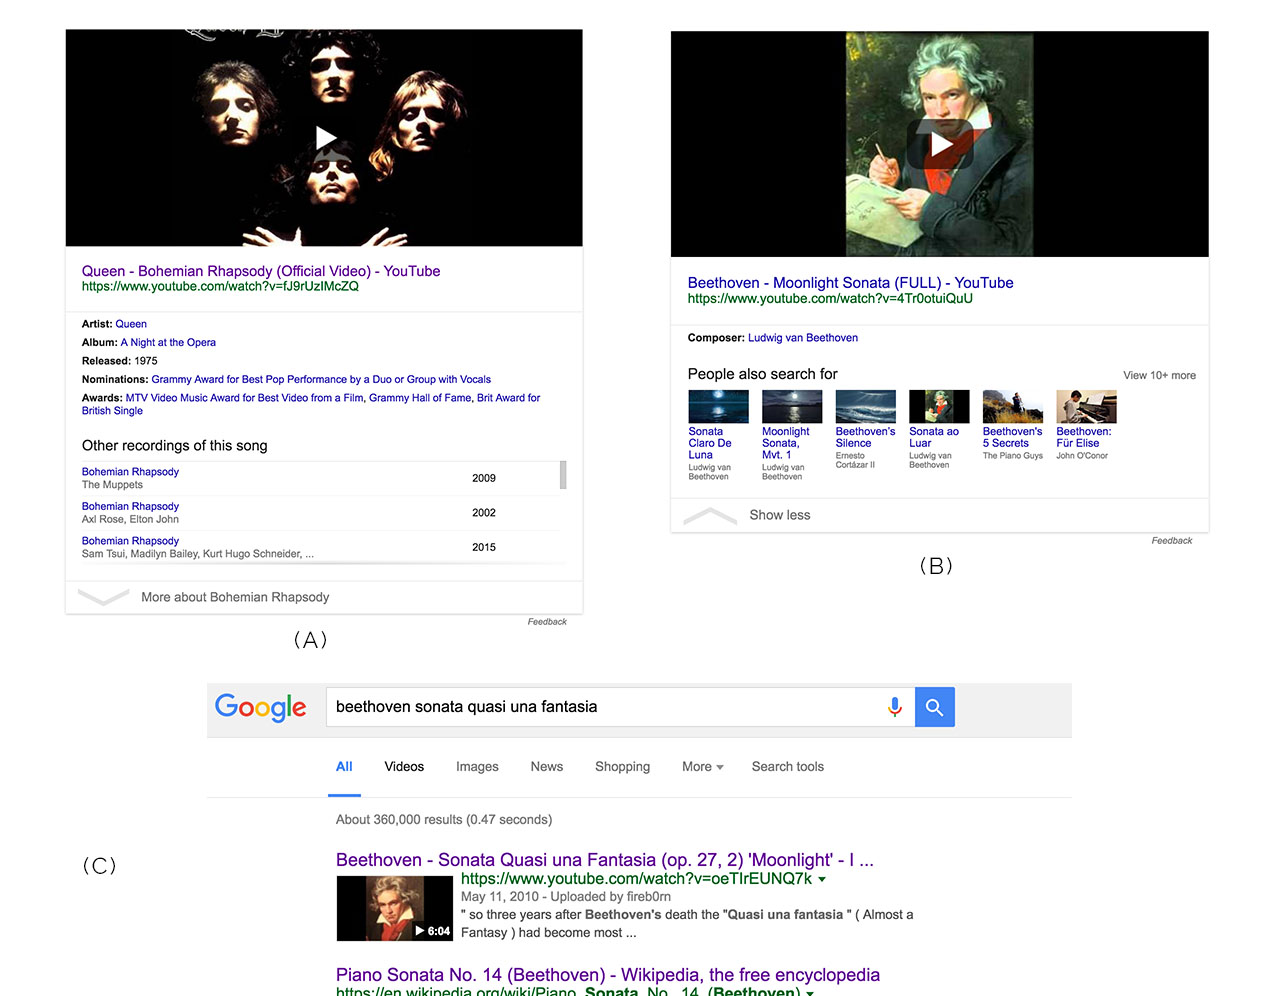
\includegraphics[width=10cm]{img/knowledge-graph.jpg}
\centering
\caption{Google's Knowledge Graph comparison: (a) result for ``Queen Bohemian Rhapsody'', (b) result for ``Beethoven Moonlight Sonata'', (c) result for ``Beethoven Sonata Quasi una Fantasia''}
\label{fig:knowledge-graph}
\end{figure}

Creative works, and in particular musical works, are complex objects. Ample information related to single works, that involves the original idea of the composer, the physical manifestation, the events of the creation and of the performances are available. For this reason, complex ontologies are required for expressing this multifaceted data, like FRBRoo and DOREMUS. As consequence of this complexity, the consumption of these ontologies by search engines and external applications is not easy. In this paper, we provide a strategy for translating a complex ontology into the \textit{de facto} standard in Structured Data for the web, Schema.org and we show how complex metadata can then be more easily consumed by search engines. We choose as starting point the representation of music made by the DOREMUS ontology.

In Section \ref{sec:background}, we describe briefly the FRBRoo extension, its extension for music, DOREMUS, and Schema.org. Section \ref{sec:simplification} contains some recipes for executing the mapping. The result of the mapping is evaluated in Section \ref{sec:evaluation}. In Section \ref{sec:conclusion} we conclude with an example of an app for visualizing Schema.org metadata.

%%%%%%%%%%%%%%%%%%%%%%%%%%%%%%%%%%
%%%  2. Background Ontologies  %%%
%%%%%%%%%%%%%%%%%%%%%%%%%%%%%%%%%%

\section{Background Ontologies}
\label{sec:background}
In this section, we first describe the two models we want to map: the DOREMUS ontology for music and Schema.org. In addition, we present briefly existing methodologies for mapping Schema.org with other ontologies and with FRBR.

\subsection{Describe bibliographic information: FRBRoo}

The International Federation of Library Associations and Institutions (IFLA) published for the first time in 1998 the Functional Requirements for Bibliographic Records (FRBR). This model describes a literary entity at 4 levels: the Works as it is in the author mind, the way in which it is realized or Expression, its materializing in a  Manifestation and a single exemplar or Item of the manifestation. Another model, the CIDOC Conceptual Reference Model (CRM), has been developed for describing information about cultural objects, focusing the attention on the process of creation of the cultural entity.

From the harmonization of FRBR and CIDOC-CRM, an ontology for describing bibliographic and museum information has born with the name FRBRoo \cite{doerr2008frbroo}. It presents a model for describing arts from a documentation perspective.

The central feature of the ontology is the presence of the triplet of classes Work - Event - Expression: every artistic Work, exists only through an Event of creation, that realizes the Work itself into an Expression. Thinking as example to the book \textit{Moby Dick}, the artistic object takes birth when the idea (Work) of the author Melville are written (Event) in the succession of words (Expression). The relations between these classes and the relative subclasses represent one of the strength of the model thanks to the wide expressiveness gained from this. In FRBRoo, one can link a work with another one one (one specific critic edition or the French translation), add more details about the creation event (where and when it took place), add derivatives works (the 1956's movie \textit{Moby Dick}) or works that are components of a complex one (the critics essays contained in a particular edition).

\subsection{An ontology for music libraries: DOREMUS}
DOREMUS\footnote{\url{http://www.doremus.org/}} is a research project that aims to develop tools and methods to describe, publish, connect and contextualize music catalogues on the web of data. In this project, an ontology \cite{achichidoremus} has been created that extends the FRBRoo model. The DOREMUS ontology adds to FRBRoo additional classes and properties that are important in the description of music works, like the key, the genre, or the intended casting of a performance. The DOREMUS model contains today 149 classes and 346 properties.

\begin{figure}
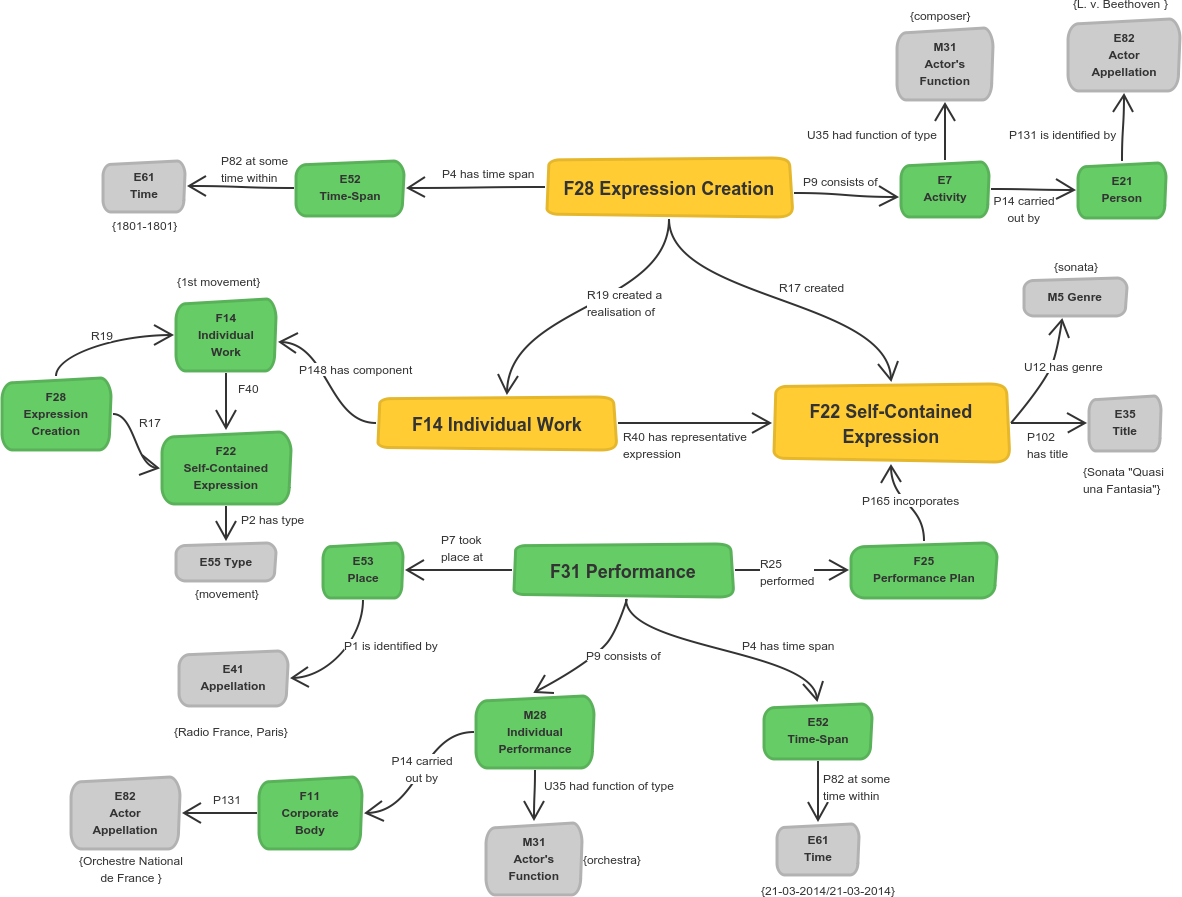
\includegraphics[width=10cm]{img/Beethoven-Doremus.png}
\centering
\caption{Graph of Beethoven's \textit{Sonata ``Quasi una Fantasia"} described through the DOREMUS ontology.}
\label{fig:beet-doremus}
\end{figure}

Figure \ref{fig:beet-doremus} shows a representation of Beethoven's \textit{Sonata ``Quasi una Fantasia"}\footnote{\url{https://en.wikipedia.org/wiki/Piano_Sonata_No._14_(Beethoven)}} using the DOREMUS ontology. It contains the description of the creation of the work in 1801, the presence of movements and an associated performance taken in Paris. The central part consists of the three main classes \textit{F28 Expression Creation}, \textit{F14 Individual Work}, \textit{F22 Self-Contained Expression}, in yellow. The nodes in green represent resources, while the gray nodes identifies some particular classes that corresponds to \textit{E59 Primitive Value}, \textit{E41 Appellation}, \textit{E55 Type} or any of their subclasses. These three groups will be further explored in Section \ref{sec:simplification}.

\subsection{Schema.org and its mappings to other ontologies}
By the initiative of some of the most popular search engines in the world, a vocabulary for structured data for web pages has been created with the name of Schema.org\footnote{\url{http://schema.org/}} \cite{guha2015schema}. The aim of this community project is to enable search engines to have a semantic understanding of the content in the web page. In order to get this, web pages should refer to the vocabulary through Microdata, RDFa or JSON-LD. Schema.org provides classes for describing persons, organizations, places, products, etc. For our purpose, the most interesting classes are CreativeWork and Event, and their subclasses. Among them, there are some music-specific classes: MusicComposition, MusicRecording, MusicEvent, MusicGroup, etc.

In the past, the community group took under consideration the possibility of modelling the structure of the CreativeWork class on the basis of FRBR, until their final resolution of avoiding it. The reason of this decision can be found in the difference of purpose of the two ontologies: FRBR is specific for describing cultural works and expressions, while Schema.org provides a way to markup a web page so that search engine can understand and use their content. According to Richard Wallis, Chair of the W3C Schema Bib Extend working group, ``replicating the FRBR rules within the [generic] Schema.org vocabulary was much discussed in the Schema Bib Extend Community Group [...] It was concluded that reproducing those rules would be too complex''\footnote{Richard Wallis, 2016 \url{https://lists.w3.org/Archives/Public/public-schemaorg/2016Feb/0024.html}}.

Nogales et al. \cite{nogales2013exploring} explored a mapping between Schema.org terms and the vocabularies collected by the Linked Open Vocabularies (LOV) project. This mapping has been realized in two steps: firstly matching classes which have exactly the same name; then, taking in account the mapped classes, matching their properties in the same way. The mapping has been developed in \cite{nogales2016linking} through the use of dictionaries: a mapping exists if names of the classes involved are exactly the same or have a synonym in common. An additional manual check confirm the goodness of the match.

Speaking of DOREMUS (or FRBRoo, in general), we cannot use this approach for extracting matches. With few exceptions (e.g. Event, PublicationEvent), the involved ontology and Schema.org have no classes with exactly the same name. Also, matching similar names could be wrong: the DOREMUS ``F1 Work'' and ``CreativeWork'', in its subclass ``MusicComposition'', match if we consider the names, but some properties that belong to the latter, like title/name, [musical]Key and genre, are not attached to a ``F1 Work'', but to a ``F2 Expression''.

In \cite{godby2013relationship} a solution is introduced for expressing FRBR entities using concepts that belongs to Schema.org. This work proposes to map each level of the chain Work - Expression - Manifestation - Item with a entity of the CreativeWork class. A limit of this strategy is that the information is split up among different objects. On one side it expresses exactly the librarian concepts contained in FRBR, but on the other hand, when one searches for the Beethoven's Sonata, one should also consider if it is the Work (with properties such as author or creation date) or the Expression (with properties such as genre and key) which is being searched. How to find the most suitable match between classes of the two ontologies? How about concepts that are not in the target ontology? We aim to answer to those questions in the following section, by providing some recipes that enable to benefit from schema.org while starting from a more complex ontological model.

%%%%%%%%%%%%%%%%%%%%%%%%%%%%%%%%%
%%%  3. Model simplification  %%%
%%%%%%%%%%%%%%%%%%%%%%%%%%%%%%%%%

\section{Model simplification}
\label{sec:simplification}
In this section, the broad expressiveness of the DOREMUS ontology will be mapped into a less specific ontology, with the purpose of improving search results and experience on search engines. Starting from the example of Beethoven's \textit{Sonata ``Quasi una Fantasia"} expressed with the DOREMUS model (Figure \ref{fig:beet-doremus}), we aim to represent the same information using Schema.org. We expect to map the nodes marked in gray with a literal value of a Schema.org property, while yellow and green nodes with a class.

The method is based on the observation of the graph. The main idea is to identify a suitable starting node and progress following the links until the graph borders. This method assumes a sufficient knowledge of the models that are going to be mapped, and is structured as a series of recipes to follow. We refer to DOREMUS or FRBRoo classes and properties using the prefix ``mus" (e.g. \textit{mus:F1 Work}) and to Schema.org ones with ``sdo" (e.g. \textit{sdo:CreativeWork}).

\subsection{Choose the starting node}
The most suitable starting point should coincide with the most significant class or group of classes in the starting ontology, DOREMUS. There are different way for evaluate it. As an example, it could be the class with the highest number of occurrences, as this can be evaluated by tools like LOUPE \cite{mihindukulasooriya2015loupe}. Another strategy could rely on the recognition of a frequent pattern in the ontology, like the Work-Expression-Event triangle in FRBRoo.

As a consequence, the choice will consider what we expect that people are going to search, reasonably textual queries like ``Sonata Quasi una Fantasia'' or ``Beethoven Sonata Quasi una Fantasia''. According to this, information about title and author gains a key role. We choose as starting node \textit{mus:F2 Expression} that has the properties \textit{mus:P102 has title}, and \textit{mus:F28 Expression Creation} because of its link with the information about the composer.

\subsection{Identify similar classes}
\label{sec:classmap}
We start to match the classes, starting form the ones we identified in the previous step. For each class in the source model (DOREMUS), we search the best class that can represent it in the target model (Schema.org), trying to respect one or more of these criteria:
\begin{enumerate}
 \item{
They should have similar name.\newline
e.g. \textit{mus:F28 Expression Creation} $\rightarrow$ \textit{sdo:CreateAction}.
}
 \item{They should have similar description}
 \item{They should have similar properties\newline
e.g. \textit{mus:F2 Expression U11 has key} $\rightarrow$ \textit{sdo:MusicComposition.musicalKey}
}
 \item{They should have similar properties value expected\newline
e.g. \textit{mus:F2 Expression U12 has genre} and \textit{sdo:MusicComposition.music-CompositionForm} have both “sonata” as possible value}
\end{enumerate}

The matches that better satisfy the criteria are: \textit{mus:F28 Expression Creation} $\rightarrow$  \textit{sdo:CreateAction} and \textit{mus:F2 Expression} $\rightarrow$  \textit{sdo:MusicComposition}.

\subsection{Identify similar properties}
    \label{sec:propmap}
For each class mapped, a mapping between properties should be performed. The criteria are similar to the previous ones:
\begin{enumerate}
\item{
 They should have similar name.\newline
e.g. \textit{mus:U11 has key} $\rightarrow$ \textit{sdo:musicalKey}
}
 \item{They should have similar description}
 \item{They should have similar value expected\newline
e.g. \textit{mus:U12 has genre} and \textit{sdo:musicCompositionForm} have both “sonata” as possible value}
\end{enumerate}

Each mapped property could have as value a literal (e.g. key, genre and all the ``gray'' nodes in Figure \ref{fig:beet-doremus}) or another class  (e.g. the composer is a Person). In the latter case, if we have not previously mapped this class, we consider it as a new input for steps \ref{sec:classmap} and \ref{sec:propmap}, until every node in the graph has been reached.

The result of a complete iteration of \ref{sec:classmap} and \ref{sec:propmap} is a set of classes and properties mapped, so that a new graph could be drawn (Figure \ref{fig:beet-inter}). It shows that \textit{sdo:MusicComposition} is repeated multiple times, each one with different linked information, depending on the fact that it maps a Work or an Expression.

\begin{figure}
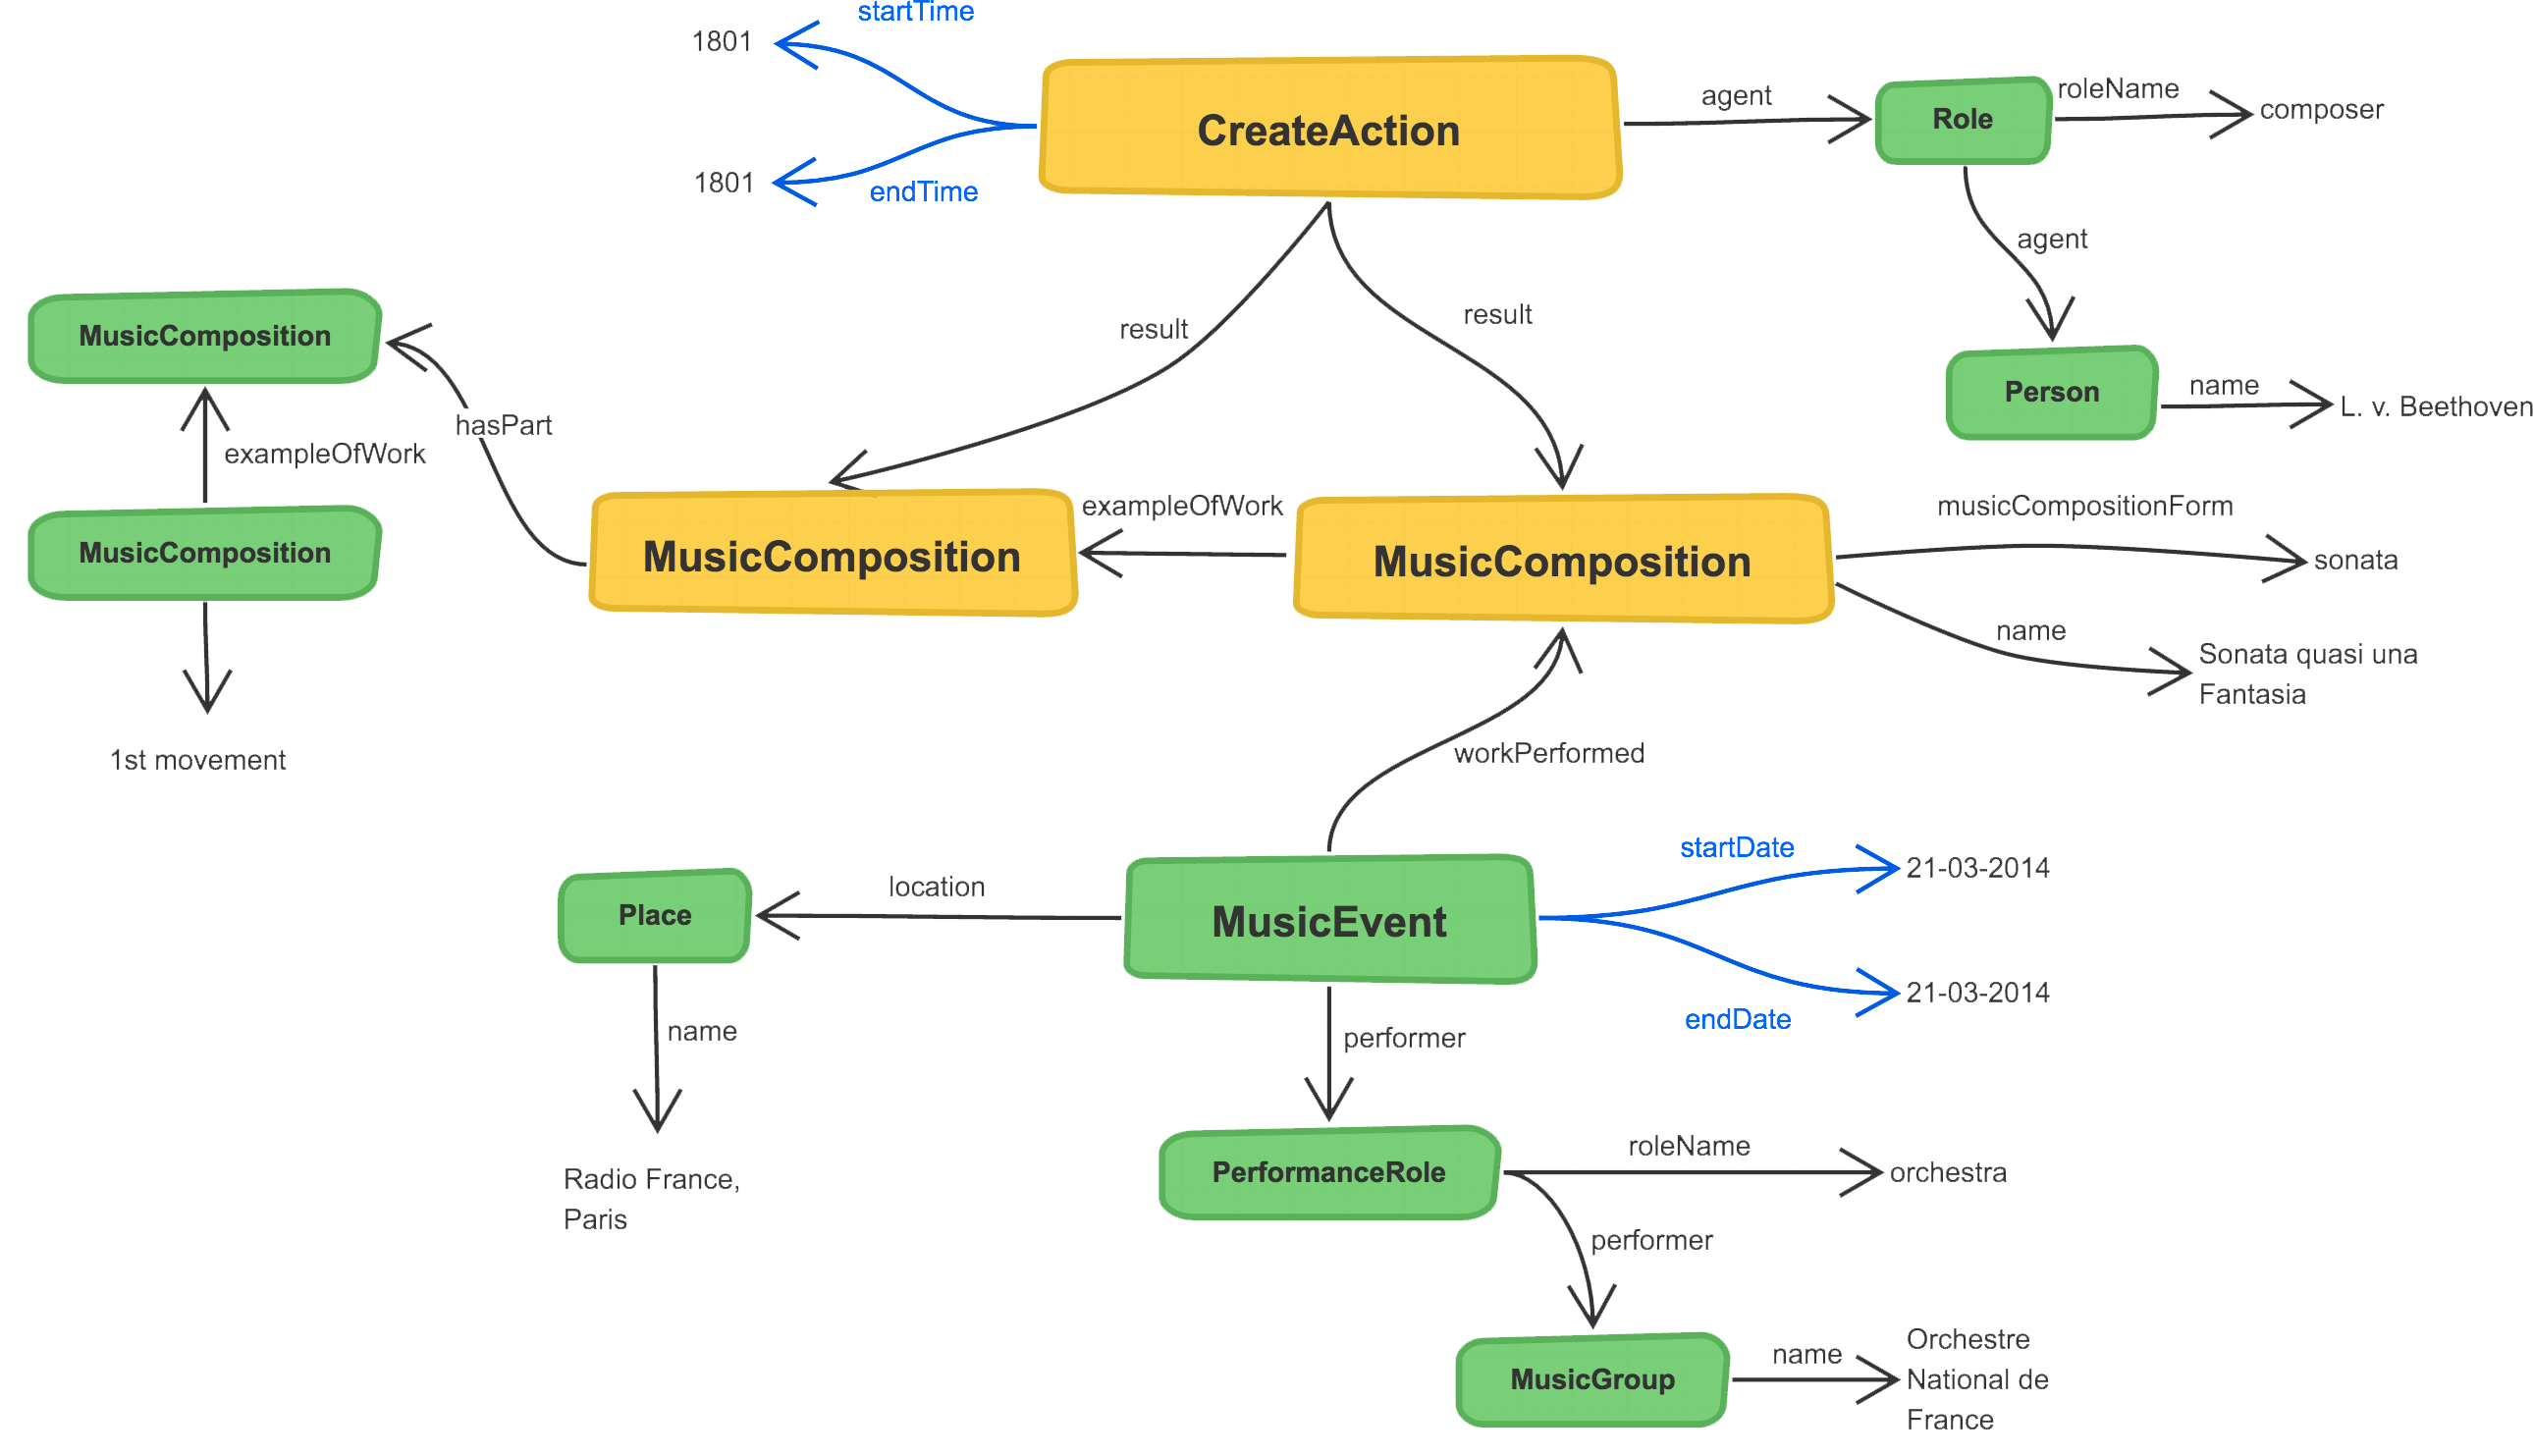
\includegraphics[width=12cm]{img/beethoven-intermediate.png}
\centering
\caption{Graph of Beethoven's \textit{Sonata ``Quasi una Fantasia"} after the first phases of mapping to Schema.org.}
\label{fig:beet-inter}
\end{figure}

\subsection{Simplify the graph}
\begin{figure}
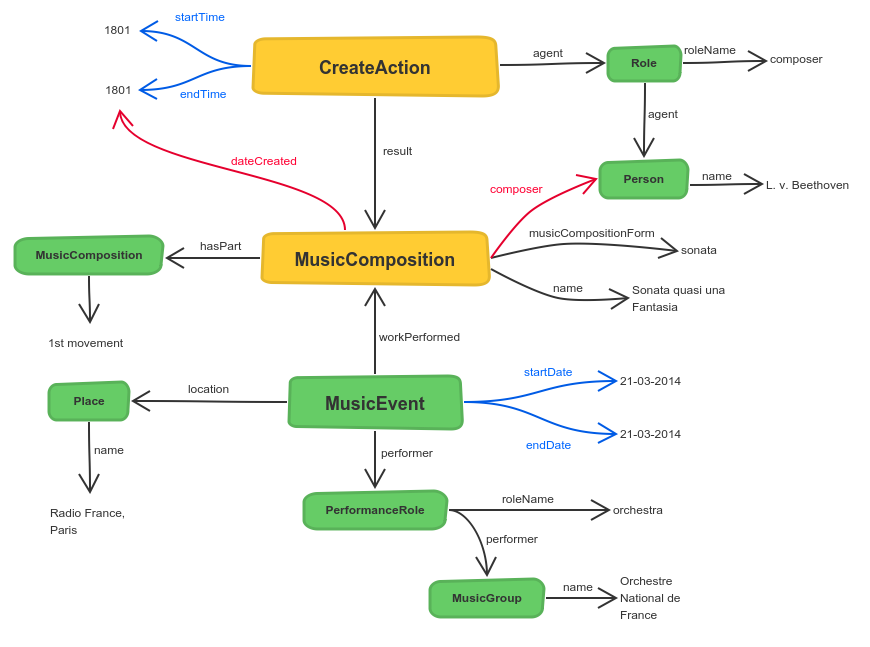
\includegraphics[width=12cm]{img/Beethoven-Schema.png}
\centering
\caption{Graph of Beethoven's \textit{Sonata ``Quasi una Fantasia''} described through Schema.org.}
\label{fig:beet-schema}
\end{figure}

Merging these nodes can produce the advantage of a simpler model, in which the information is distributed in as less nodes as possible. Such an achievement is positive for the consumption by search engines, that can display more information in a single search result. In order to do this, we identified some criteria for discerning good candidates for the merging. These criteria should not be considered as strict rules, but as common behaviors of the redundant classes.

Two nodes are redundant when:
\begin{enumerate}
\item{
They represents the same class or have a superclass in common in the target model (this criterion is required).
}
\item{
If they are both connected to a class, the connections are both realized with the same properties.\newline
e.g. \textit{mus:F1 Work} and \textit{mus:F2 Expression} are both mapped with \textit{sdo:Music-Composition} and both are connected to \textit{sdo:CreateAction} with the property \textit{sdo:result}.
}
\item{
They are connected between them.
}
\item{
They have not properties in conflict (this criterion is required). \newline
e.g. They could not have different names or keys.
}
\item{
The effect of merging does not produce any upset of the graph except a simplification.
}
\end{enumerate}

The \textit{mus:F1 Work} and \textit{mus:F2 Expression}, both mapped with \textit{sdo:Music-Composition}, satisfy all these criteria. Moreover, we consider also that the difference of these two classes is slight since from the source ontology. As a consequence, the distinction between Work and Expression is simply not relevant to the Schema.org view: users simple search for a book, a movie, a music composition, without taking in consideration the separation between the idea and the realization \cite{godby2013relationship}.

Redundant nodes are substituted with a new node with:
\begin{enumerate*}
\item{The same class of the original ones (or the most specific among the two)}
\item{The sum of their properties.}
\end{enumerate*}

The result of this phase is a new graph as it is show in Figure \ref{fig:beet-schema}. It is evident that the new graph has a simpler structure, because of the merging, the omission of some details (i.e. the part is no more marked with type "movement"), and the replacing of some nodes with primitive types. \textit{mus:E52 Time Span} has been replaced with two properties, for start and for end (in blue). Instead, we mark in read some properties that in the FRBRoo model are linked to the Event and in Schema.org can be explicit also directly on the \textit{sdo:MusicComposition} class; these properties could not be discovered through our method, but they could be added \textit{a posteriori}. Table in Appendix reports the complete mapping for the properties involved in the graphs.

\subsection{Limits of the mapping}
\label{sec:limits}
%% Move to future works?

As we stated before, a complete mapping can not be gained in the context of this paper. However, we point out a set of DOREMUS concepts that have not correspondence in Schema.org ontology. Among that, we miss information about the librarian cataloging, the desired casting for the composition (is it supposed to be an orchestra or it is for piano solo?), the tempo (is it "Allegro" or "Andante"). With our strategy we simply do not consider these concept in the mapping.

Schema.org gives the possibilities to add new properties and types through its extension mechanism. Future works will investigate on understanding how identify suitable properties and classes to extend Schema.org.

%%%%%%%%%%%%%%%%%%%%%%%%
%%%  4. Evaluation   %%%
%%%%%%%%%%%%%%%%%%%%%%%%

\section{Evaluation}
\label{sec:evaluation}

In order to evaluate the goodness of the mapping, we prepared a JSON-LD (JavaScript Object Notation for Linked Data) version of the \textit{Sonata Quasi Una Fantasia}.
{\scriptsize
\begin{verbatim}
{
    "@context": "http://schema.org",
    "@id": "http://data.doremus.org/Self_Contained_Expression/F22/3908d595",
    "@type": "MusicComposition",
    "name": "Sonata quasi una Fantasia",
    "alternateName": [
        "Sonate au clair de lune",
        "Clair de lune",
        "Sonate no 14 en do dièse mineur"
    ],
    "mentions": "Contesse Giulietta",
    "musicalKey": "Do dièse mineur",
    "musicCompositionForm": "sonate",
    "timeRequired": "PT16M",
    "description": "opus 27, n°2",
    "genre": "Musique Romantique",
    "composer": {
        "@id": "http://data.doremus.org/composer/beethoven"
    }
}
\end{verbatim}
}

The complete version of the JSON-LD file is available at \url{https://db.tt/em0GxWbT} while a more extended version (with more properties mapped) is available at \url{https://db.tt/JZkB5eeP}.

Firstly, we take advantage of two well-known Schema.org data parser: the Structured Data Testing Tool by Google\footnote{\url{https://search.google.com/structured-data/testing-tool}} and the Structured Data Linter\footnote{\url{http://linter.structured-data.org/}}. Both the tools show the structure of the Schema.org graph like a tree, with 76 statements correctly recognized. The Structured Data Linter offers in addition a preview of the result as they could be shown in a SERP, with descriptions, images, dates and so on.

\begin{figure}
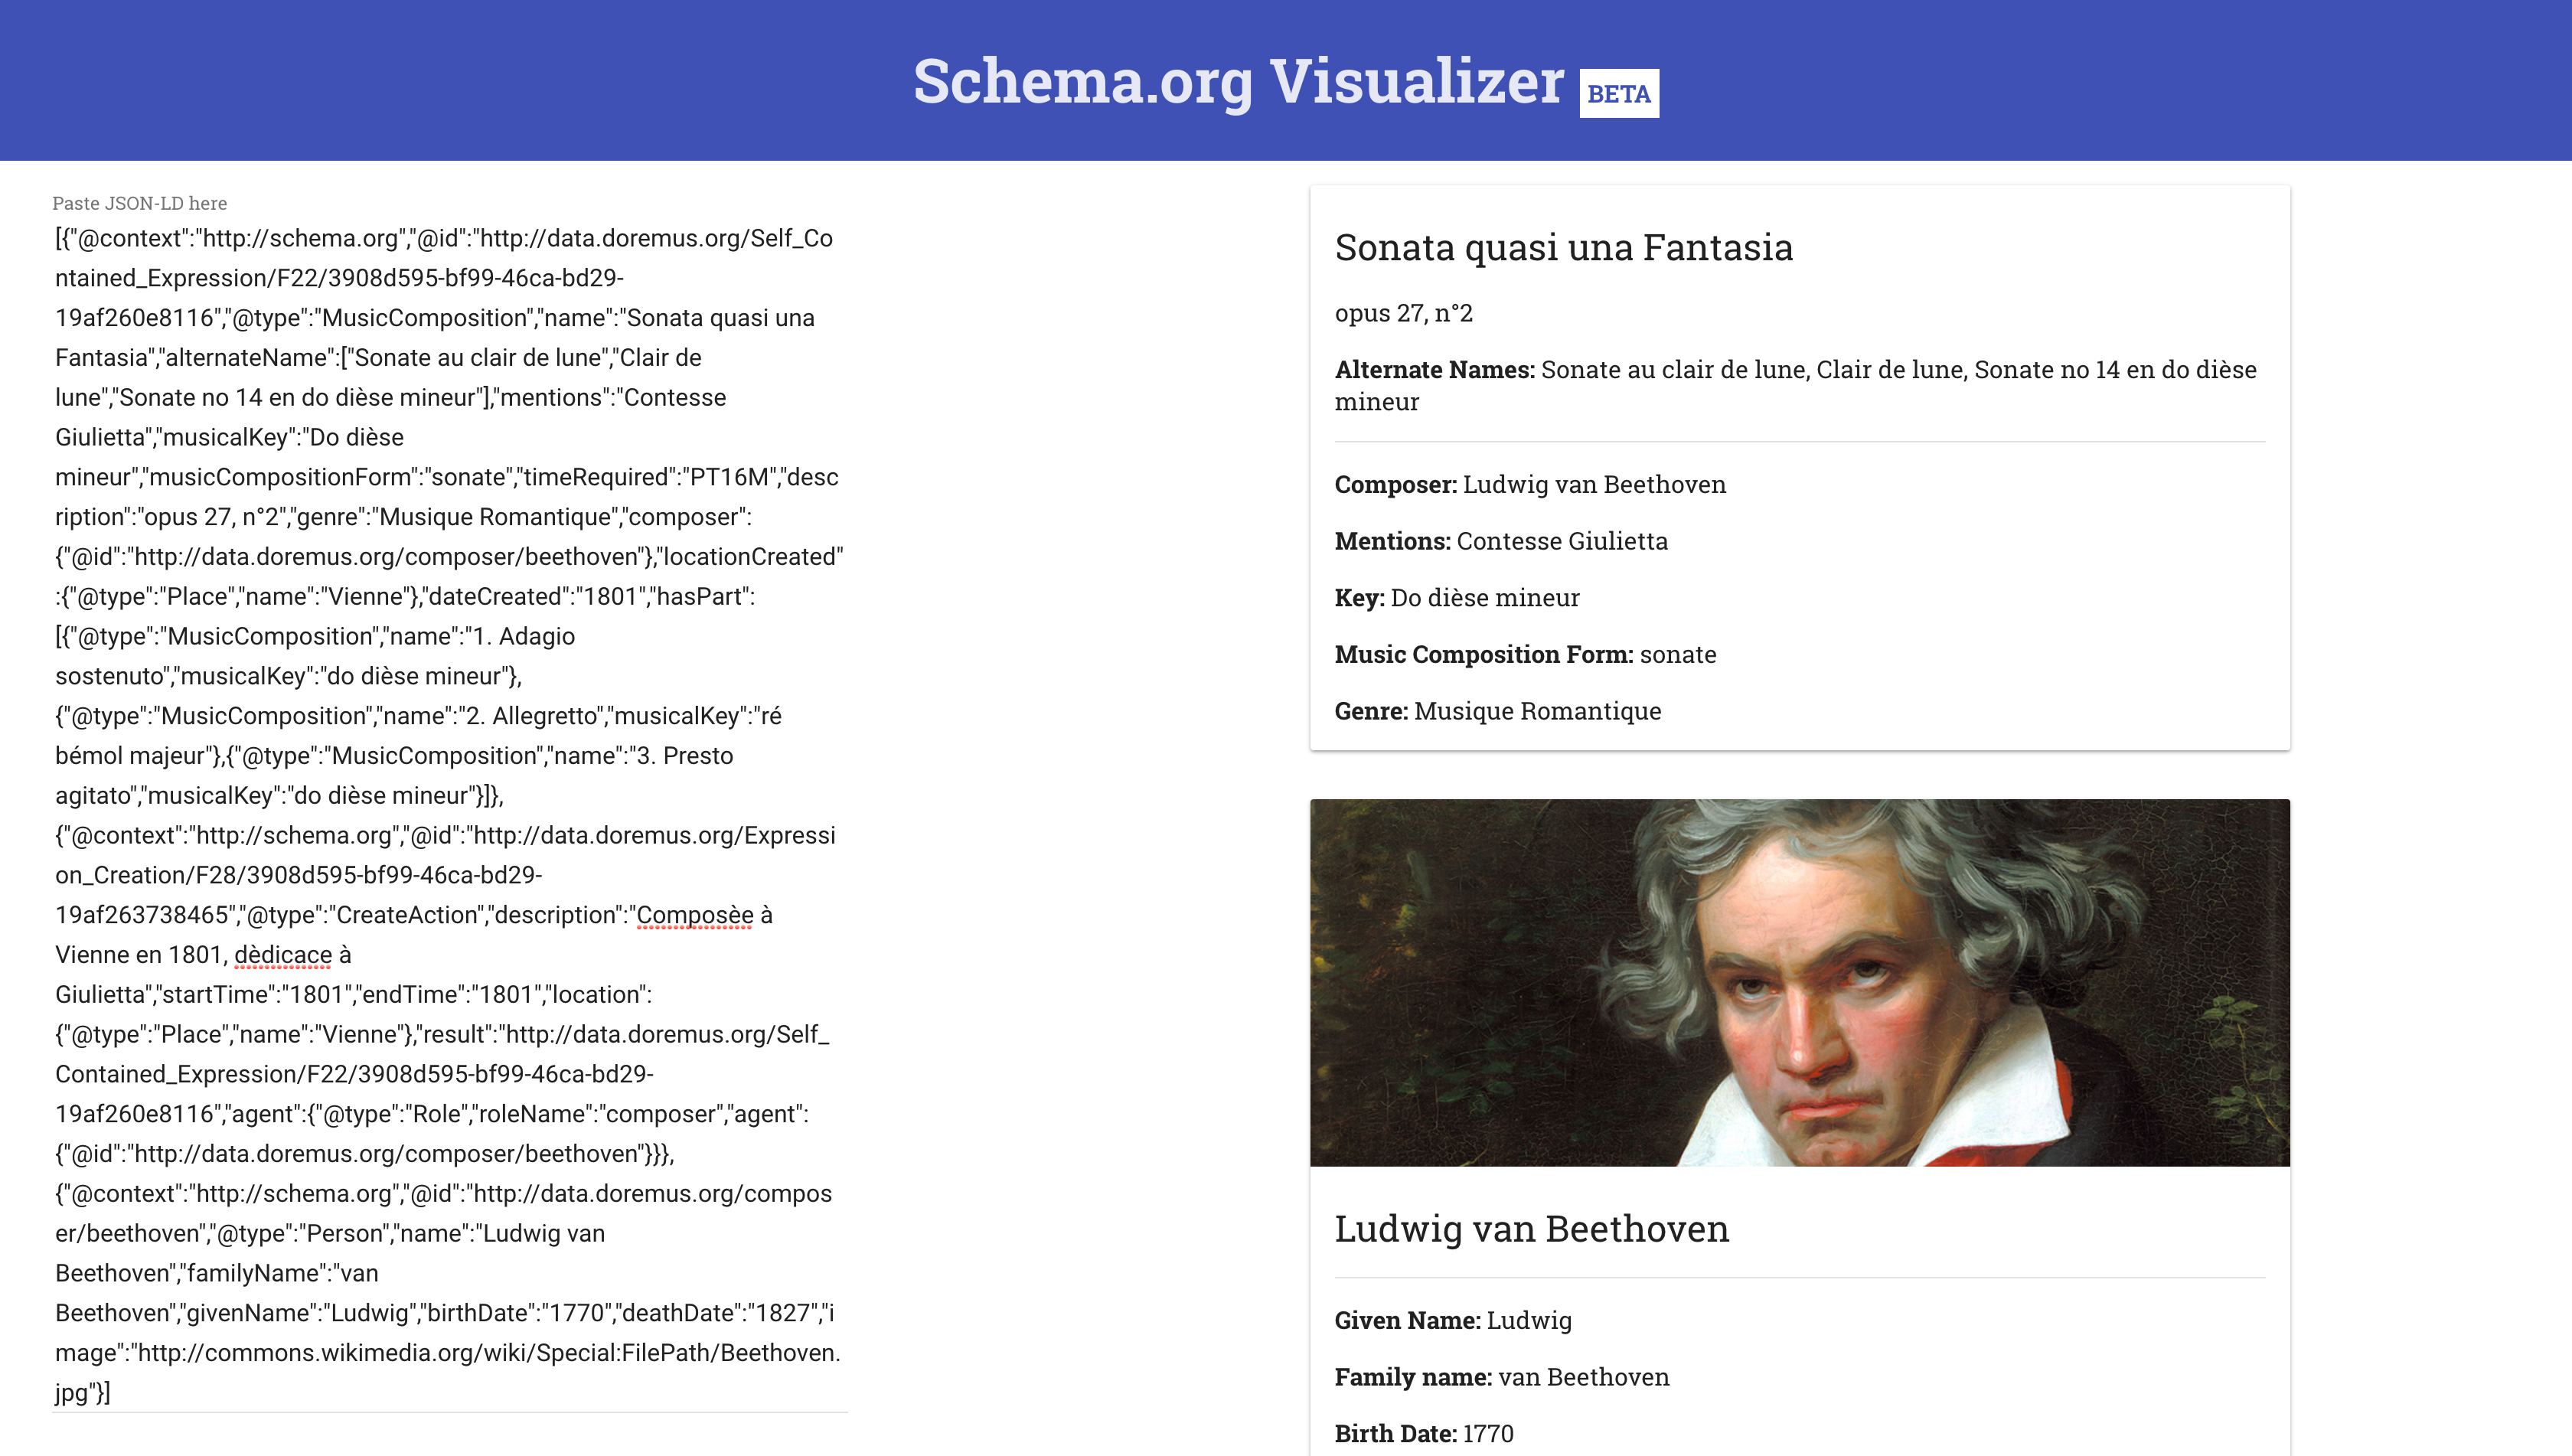
\includegraphics[width=12cm]{img/schema-visualizer.png}
\centering
\caption{The JSON-LD version of Beethoven's \textit{Sonata ``Quasi una Fantasia"} as it is parsed by Schema.org Visualizer.}
\label{fig:schema-visualizer}
\end{figure}

For having a stronger visual feedback, we developed a lightweight web application, named Schema.org Visualizer\footnote{Still in beta while we are writing this paper. \url{https://github.com/pasqLisena/schema-visualizer}}. The app, completely realized in AngularJS, consumes the data in the JSON-LD, and shows a suitable knowledge card for each node of the graph. The result for our example is shown in Figure \ref{fig:schema-visualizer}. The cards are similar to the Knowledge Graphs by Google, because our aim is to emulate what a user could find for real when searching for a musical work.


%%%%%%%%%%%%%%%%%%%%%%%%%%%%%%%%%%%%%%%
%%%  5. Conclusion and Future Work  %%%
%%%%%%%%%%%%%%%%%%%%%%%%%%%%%%%%%%%%%%%

\section{Conclusion and Future Work}
\label{sec:conclusion}

We have described a general methodology for mapping a complex ontology to a simpler one, and we have presented it in the form of a series of recipes. We applied this methodology to a FRBRoo extension for music, DOREMUS, in order to express classical music metadata as structured data in Schema.org. The final result is a compromise between expressivity and simplicity, with the goal of providing the best experience for the final user, not only in the context of Search Engines. We tested a mapped object, Beethoven's \textit{Sonata ``Quasi una Fantasia"}, with some popular structured data parser and with a lightweight app that we developed for visualizing Schema.org metadata.

We plan to carry out an exhaustive evaluation of our approach by using the recipes widely in DOREMUS and in different ontologies, considering the effect of each criterion in identifying the correct match between classes and properties. A further subject of study is the generation of an algorithm that, starting from the recipes, identifies the best candidates for mapping, as well as classes and properties that are excluded in this process.

About this, we already pointed out in \ref{sec:limits} the possibility of collect these excluded elements in order to propose a musical extension for Schema.org or for the \textit{bib.schema.org} extension. An accurate selection of this information needs to be make, taking care of separating elements that could be interesting for the activity of searching and less relevant ones, in the respect of the Schema.org main goal of making the web better consumable by Search Engines and, as a consequence, by the final user.

The result of the mapping described in this paper will be soon integrated in a web application for the exploration of musical data, realized in the context of the DOREMUS project.

\section*{Acknowledgments}
This work has been partially supported by the French National Research Agency (ANR) within the DOREMUS Project, under grant number ANR-14-CE24-0020.

% ---- Bibliography ----
\bibliographystyle{abbrv}
\bibliography{bib-doremus}

\newpage

\section*{Appendix: Mapping-table from DOREMUS to Schema.org}
\label{sec:table}

The following Table shows the mapping rules for DOREMUS, extracted through the method described in this paper.

\tablehead{
\textbf{DOREMUS} \newline Property $\rightarrow$ Class
&
\textbf{Schema.org} \newline Property $\rightarrow$ Class\\\hline
}
\tabletail{\hline {Continued on next page} \\}
\tablelasttail{\hline \hline}
\begin{center}
\setlength{\tabcolsep}{10pt}
\renewcommand{\arraystretch}{1.7}
\label{tab:map}
\begin{xtabular}{p{6.7cm} p{4cm} }
% F2 EXPRESSION
\multicolumn{2}{c}{mus:F2 Expression $\rightarrow$ sdo:MusicComposition}\\
\hline
P102 has title $\rightarrow$ E35 Title
& name $\rightarrow$ Text \\
P67 refers to $\rightarrow$ M15 Dedication
& mentions $\rightarrow$ Text \\
U11 has key $\rightarrow$ M4 key
& musicalKey $\rightarrow$ Text\\
U12 has genre $\rightarrow$ M5 genre
& musicCompositionForm\newline$\rightarrow$ Text\\
U19 has style $\rightarrow$ M19 Style
& genre $\rightarrow$ Text\\
R9i realizes $\rightarrow$ F1 Work
& exampleOfWork\newline$\rightarrow$ MusicComposition\\
U4 had princeps publication\newline$\rightarrow$ F30 Publication Event
& publication\newline$\rightarrow$ PublicationEvent\\
P165i is incorporated in\newline$\rightarrow$ F24 Publication Expression
& publication\newline$\rightarrow$ PublicationEvent\\
R24i was created through\newline$\rightarrow$  F24 Publication Event
& publication\newline$\rightarrow$ PublicationEvent\\
% F1 Work
\hline
\multicolumn{2}{c}{mus:F1 Work $\rightarrow$ sdo:MusicComposition}\\
\hline
P148 has component \newline$\rightarrow$ F14 Individual Work
& hasPart \newline$\rightarrow$ MusicComposition\\
% F28 EXPRESSION CREATION
\hline
\multicolumn{2}{c}{mus:F28 Expression Creation $\rightarrow$ sdo:CreationEvent}\\
\hline
P4 has time span\newline $\rightarrow$ E52 Time-span
& startTime $\rightarrow$ Date \newline
endTime $\rightarrow$ Date\newline
\textit{(split into 2 properties)} \\
R17 created\newline$\rightarrow$ F22 Self-Contained Expression
& result\newline $\rightarrow$ MusicComposition\\
P9 consists of $\rightarrow$ E7 Activity
& agent $\rightarrow$ Role\\
% E7 Activity
\hline
\multicolumn{2}{c}{mus:E7 Activity $\rightarrow$ sdo:Role}\\
\hline
U35 had function of type \newline $\rightarrow$ M31 Actor's Function
& roleName $\rightarrow$ Text \\
R14 carried out by\newline$\rightarrow$ E21 Person
& [inital property]\newline $\rightarrow$ Person\\
% E21 Person
\hline
\multicolumn{2}{c}{mus:E21 Person $\rightarrow$ sdo:Person}\\
\hline
P135 is identified by \newline $\rightarrow$ E82 Actor Appellation
& name $\rightarrow$ Text \\
% E53 Place
\hline
\multicolumn{2}{c}{mus:E53 Place $\rightarrow$ sdo:Place}\\
\hline
P1 is identified by \newline $\rightarrow$ E41 Appellation
& name $\rightarrow$ Text \\
% F11 Corporate Body
\hline
\multicolumn{2}{c}{mus:F11 Corporate Body $\rightarrow$ sdo:MusicGroup}\\
\hline
P135 is identified by \newline $\rightarrow$ E82 Actor Appellation
& name $\rightarrow$ Text \\
% F31 Performance
\hline
\multicolumn{2}{c}{mus:F31 Performance $\rightarrow$ sdo:MusicEvent}\\
\hline
R25 performed $\rightarrow$ F25 Performance Plan \newline $\rightarrow$ P165 incorporates \newline $\rightarrow$ F22 Self-Contained Expression
& workPerformed \newline $\rightarrow$ MusicComposition \\
P4 has time span \newline $\rightarrow$ E52 Time-Span
& startDate $\rightarrow$ Date \newline
endDate $\rightarrow$ Date\newline
\textit{(split into 2 properties)} \\
P7 took place at $\rightarrow$ E35 Place
& location $\rightarrow$ Place \\
%
\end{xtabular}
\centering
\end{center}



\end{document}